\section{Локальные дескрипторы}

%\subsection{Простая векторизация}

\begin{frame}{Локальность признаков}

А что если мы векторизовывать будем не всё изображения, а его части?

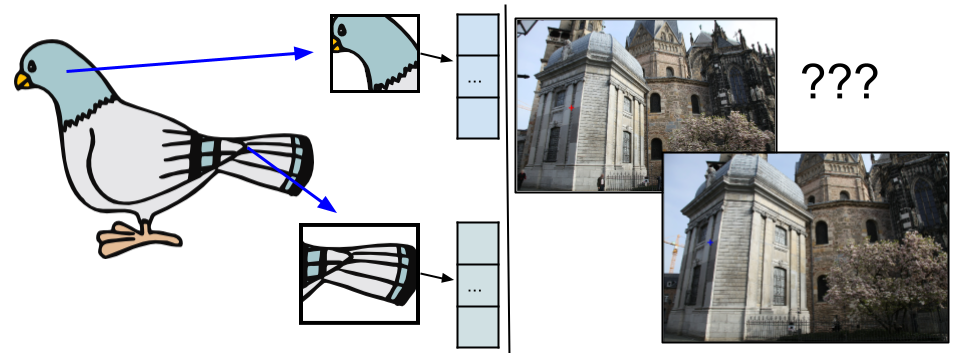
\includegraphics[width=0.9\textwidth]{images/pigeon local2.png}

Как понять, какие части изображения нам интересны?
    
\end{frame}

\begin{frame}{Особые точки}

\begin{itemize}
    \item Опишем набор особых точек: углы, локальные максимумы яркости, границы, и т.д.
    \item Теперь используя это описание будем искать такие наборы точек на нашем изображении.
\end{itemize}
\centering
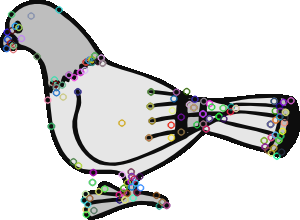
\includegraphics[width=0.3\textwidth]{images/pigeon_sift.png}
\end{frame}

\begin{frame}{SIFT-подобные дескрипторы}
Нам не достаточно находить только координаты.

\begin{tabular}{m{17em} m{20em}}
    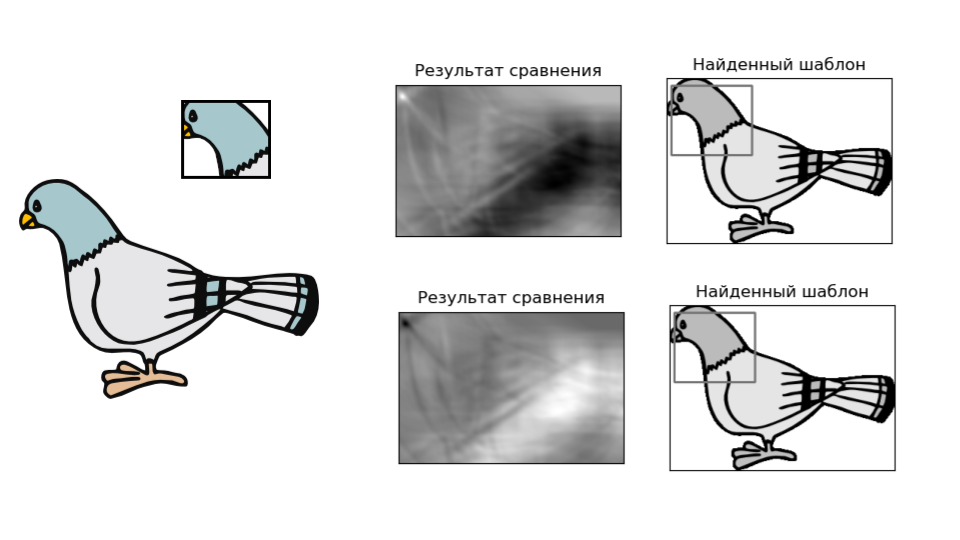
\includegraphics[width=0.5\textwidth]{images/pigeon template matching2.png} & 
    \begin{itemize}
        \item Можно использовать <<похожесть>> шаблона в качестве дескриптора точки.
        \item Ещё можно считать <<уникальность>> пикселя по сравнению с соседями.
    \end{itemize}
\end{tabular}
    
\end{frame}

\begin{frame}{Нейросети}

\begin{itemize}
    \item Если у нас есть фиксированный набор <<особенностей>>, можно обучить нейросетевой детектор.
    \item А затем дообучить его, чтобы на похожих точках он выдавал лизкие дескрипторы (SuperPoint\footfullcite{detone18superpoint}).
    \item У нас могут получиться плохие дескрипторы, давайте дополнительно оценивать <<надёжность>> (R2D2\footfullcite{r2d2})
\end{itemize}

\centering
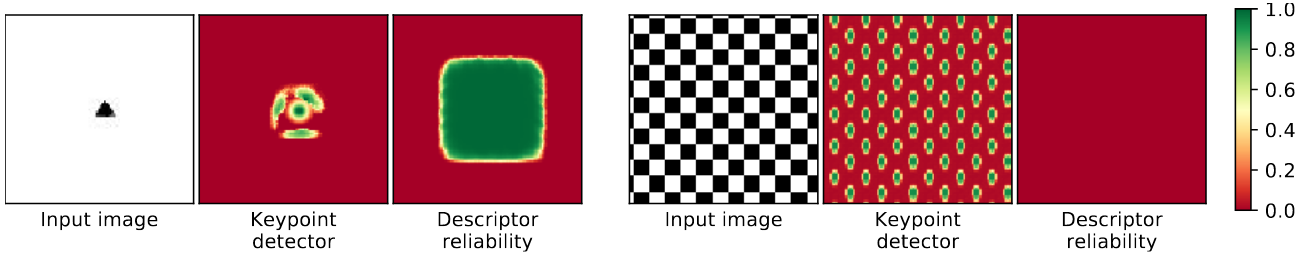
\includegraphics[width=0.9\textwidth]{images/r2d2_reliability.png}

\end{frame}

\begin{frame}{Матчинг дескрипторов}

\begin{itemize}
    \item Мы можем сравнивать дескрипторы как обычные вектора.
    \item Но чтобы сравнивать изображения надо сравнивать наборы дескрипторов друг с другом.
    \item При сравнении мы можем построить граф расстояний, и использовать его для дополнительной информации.
    \item Например обучить графовую нейросеть! (SuperGlue\footfullcite{sarlin20superglue})
\end{itemize}
    
\end{frame}
